\documentclass[11pt]{article}
%\usepackage{enumerate}
%\usepackage{fullpage}
\usepackage{graphicx}
\usepackage{amssymb}
\usepackage{amsmath}
\usepackage{subcaption}
\usepackage{bm}
\usepackage{float}
\usepackage{fancyhdr}
\usepackage{listings}
\usepackage{color}
\usepackage{hyperref}



\pagestyle{fancy}
\fancyhead{}
\fancyhead[L]{Epidemic Modeller Project Overview — Alex Gardner}
\fancyfoot{}
\fancyfoot[C]{\thepage}

\setlength{\headheight}{14pt}

\begin{document}
\title{Epidemic Modeller Project Overview}
\author{Alex Gardner}
\date{MA4J5}
\maketitle

\section*{Introduction}

\section*{Basic Visual Model}
\subsection*{Setup}
We start with a region $A=[0,1]\times [0,1]$, and each individual $i$ has coordinates $(x_i, y_i)\in A$. Each individual starts with coordinates $x_i \sim U[0,1]$, $y_i \sim U[0,1]$, and has velocity $\frac{dx_i(t)}{dt} \sim U[-v,v]$, $\frac{dy_i(t)}{dt} \sim U[-v,v]$ for some speed parameter $v$. Whenever an individual hits the boundary, e.g. $x_i=0$, then they 'bounce' off of the boundary by negating the velocity in the $x$ or $y$ component, whichever boundary we hit.

\begin{figure}[H]
\label{BasicModelDiagram}
\begin{center}
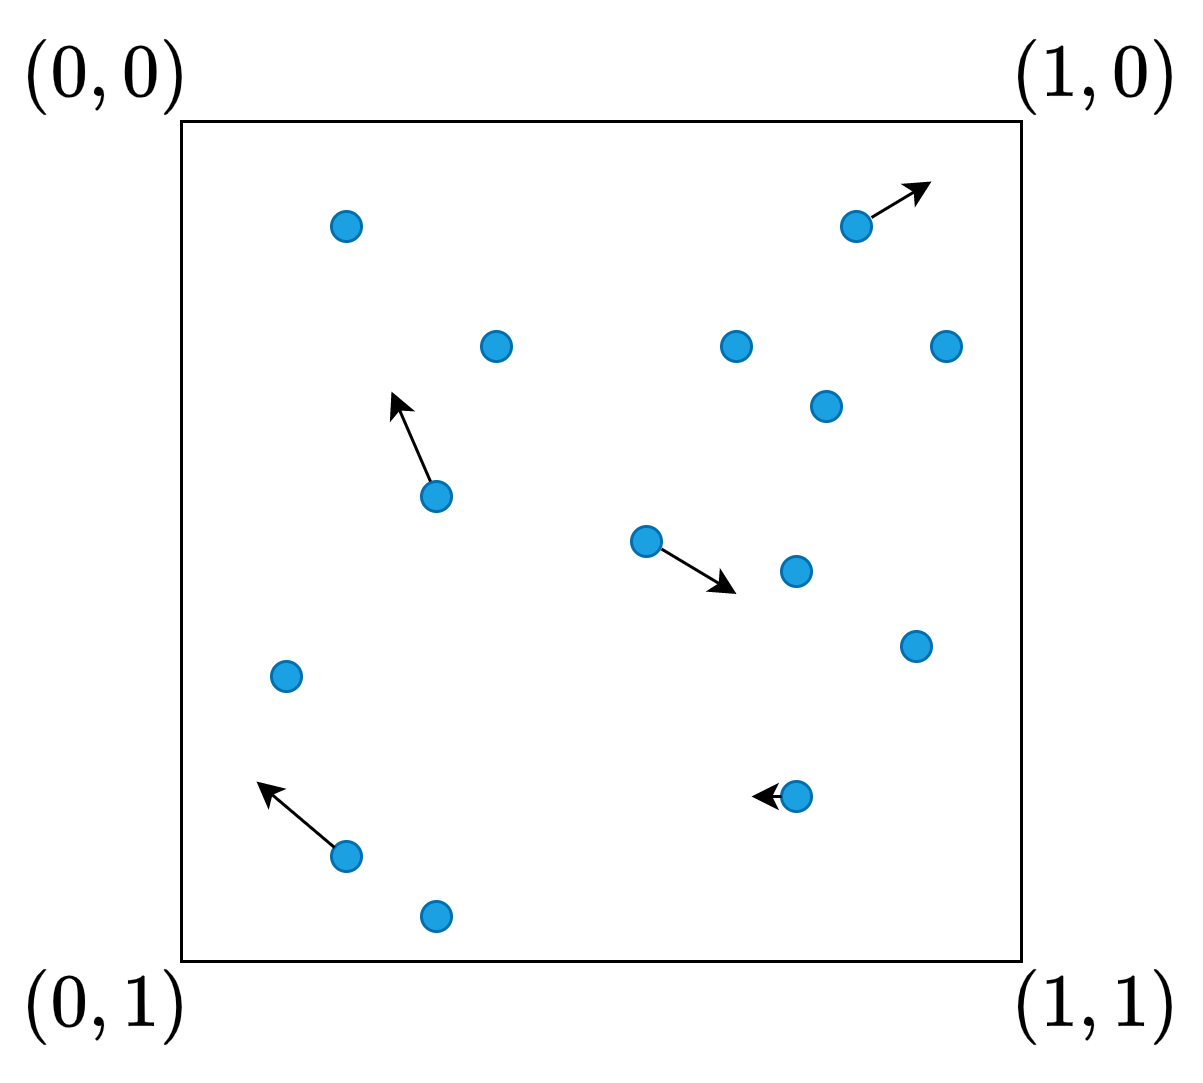
\includegraphics[width=0.6\textwidth]{BasicModelDiagram1}
\end{center}
\end{figure}

Each individual has state $s_i\in \{S,E,I,R\}$ and our model starts with $N_S$ people in the S class, $N_I$ in the I class, $N_E$ in the E class, and $N_R$ in the R class. When an individual enters the E class (after getting infected, or by initial condition), then they get assigned a time when their latency period will end, which is distributed $t_L \sim \text{Gamma}(\sigma)$. When an individual enters the I class, they get assigned a time when their infection period will end, which is distributed $t_R \sim \text{Gamma}(\frac{1}{\gamma\lambda}, \lambda)$. Also when an individual enters the I class, they get assigned a time at which they will next attempt to infect, with distribution $t_I\sim \text{Exp}(\lambda)$. Once an infectious person attempts to infect, they get assigned the next time when they will infect (with the same distribution), though they won't be able to attempt to infect any more if they recover before the time to next infect attempt.
\subsubsection*{Infect attempts}
Whenever an individual attempts to infect, we check if there is at least one other individual within $l^1$ distance $\frac{b}{\sqrt{N}}$. We choose this distance because there is $1/N$ area per individual in the region $A$, and if that were a square it would have side length $1/\sqrt{N}$, and then we just multiply that by a scalar parameter $b$ which we can choose when setting up the model. If there is no susceptible people in the area then the attempt failed and nobody new got infected. If there was at least one susceptible individual nearby, then one of them gets picked and enters the exposed class.

\subsubsection*{Analysis}
The recovery rate $\gamma$ is the inverse of the average number of days spent in the I class. Hence why time spent in the infectious class $t_R \sim \text{Gamma}(\frac{1}{\gamma\lambda}, \lambda)$ was chosen, because $\mathbb{E}(t_R)=\frac{1}{\gamma\lambda} \lambda=\frac{1}{\gamma}$.

The number of people in an $l^1$ radius $\frac{b}{\sqrt{N}}$ of an infectious individual's position would be effectively distributed with $m\sim \text{Binomial}(S,b/N)$. Hence the probability that there is at least 1 susceptible individual in that area will be $\mathbb{P}(m\geq 1) = 1-\mathbb{P}(m=0) = 1-(1-\frac{b}{N})^S$. This gives us the probability that a given infection attempt will be successful.

Approximating $R_0$: First we assume that $S\approx N$ for calculating the average number of people that the first person will infect. This allows us to simplify our above probability for a successful infection attempt $1-(1-\frac{b}{N})^S\approx 1-\exp(-b)$. For the first infectious individual, the time taken between each infection attempt is distributed $t_I\sim \text{Exp}(\lambda)$ and the time taken to recovery is $t_R \sim \text{Gamma}(\frac{1}{\gamma\lambda}, \lambda)$. This was chosen so that the average length of infection was $1/\gamma$ and because $\text{Gamma}(\frac{1}{\gamma\lambda}, \lambda)$ is effectively the sum of $\frac{1}{\gamma\lambda}$ of $\text{Exp}(\lambda)$ random variables, so the average number of infection attempts over the duration of the first infection should be $\frac{1}{\gamma\lambda}$. This means that $R_0\approx\frac{1}{\gamma\lambda}(1-\exp(-b))$. And so our contact rate $\beta$ should be approximately $\frac{1}{\lambda}(1-\exp(-b))$.

So, with this result, given a $\beta$ value, we can fix either $\lambda$ or $b$ and then calculate the value of the other parameter that we didn't fix so that $\beta = \frac{1}{\lambda}(1-\exp(-b))$.
\end{document}
